% This must be in the first 5 lines to tell arXiv to use pdfLaTeX, which is strongly recommended.
\pdfoutput=1
% In particular, the hyperref package requires pdfLaTeX in order to break URLs across lines.

\documentclass[11pt]{article}

% Remove the "review" option to generate the final version.
\usepackage[review]{acl}

% Standard package includes
\usepackage{times}
\usepackage{latexsym}
\usepackage{lipsum}
\usepackage{booktabs}
\usepackage{graphicx}

% For proper rendering and hyphenation of words containing Latin characters (including in bib files)
\usepackage[T1]{fontenc}
% For Vietnamese characters
% \usepackage[T5]{fontenc}
% See https://www.latex-project.org/help/documentation/encguide.pdf for other character sets

% This assumes your files are encoded as UTF8
\usepackage[utf8]{inputenc}

% This is not strictly necessary, and may be commented out,
% but it will improve the layout of the manuscript,
% and will typically save some space.
\usepackage{microtype}

\newcommand{\todo}[1]{\textcolor{red}{#1}}

% If the title and author information does not fit in the area allocated, uncomment the following
%
%\setlength\titlebox{<dim>}
%
% and set <dim> to something 5cm or larger.

\title{Sentiment Analysis of Turtle Books:\\A 439/539 NLP Project}

% Author information can be set in various styles:
% For several authors from the same institution:
% \author{Author 1 \and ... \and Author n \\
%         Address line \\ ... \\ Address line}
% if the names do not fit well on one line use
%         Author 1 \\ {\bf Author 2} \\ ... \\ {\bf Author n} \\
% For authors from different institutions:
% \author{Author 1 \\ Address line \\  ... \\ Address line
%         \And  ... \And
%         Author n \\ Address line \\ ... \\ Address line}
% To start a seperate ``row'' of authors use \AND, as in
% \author{Author 1 \\ Address line \\  ... \\ Address line
%         \AND
%         Author 2 \\ Address line \\ ... \\ Address line \And
%         Author 3 \\ Address line \\ ... \\ Address line}

\author{Jane Smith \\
  University of Arizona, Tucson, AZ, USA. \\
  \texttt{jane@arizona.edu} \\}

\begin{document}
\maketitle
\begin{abstract}
The abstract should be approximately 100 words, and outline the problem (1-sentence), the specific task you're working on (1-sentence), your proposed approach/solution to the task (1 to 2 sentences), and your results (1-sentence). \todo{\lipsum[4]}
\end{abstract}

\section{Introduction}

The introduction should describe the problem area that you're working on in high-level general terms and it's utility, identify that gap in knowledge/the need, and then how you address that need.  

For example: Sentiment analysis aims to automatically identify whether a piece of text is describing generally positive, neutral, or negative emotion  \textit{(the high-level description)}.  Sentiment analysis has broad utility, for example in automatically determining whether natural language comments left by consumers on online shopping platforms are expressing positive or negative emotion about particular products.  Automatically analyzing the sentiment of products can help shopping platforms identify new products with positive reviews that could be highlighted to increase sales, or allow manufacturers to quickly sift through a large number of product reviews to identify potential areas of improvement \textit{the utility of working on the task}.

Currently, there is \textit{gap in knowledge}, for example, lack of sentiment analysis for a particular subdomain (e.g. books about turtles).  In this work, we collect a dataset of 200 reviews of turtle books and provide human labels of their sentiment.  We then train a XYZ model using this dataset, showing that we can reach an overall performance of XX\% for this important task \textit{(how you address the need/the contribution)}. See Figure~\ref{fig:overview} for an example.


%
% Example trees
%
\begin{figure}[!t]
%	\vspace{-12pt}
	\centering
	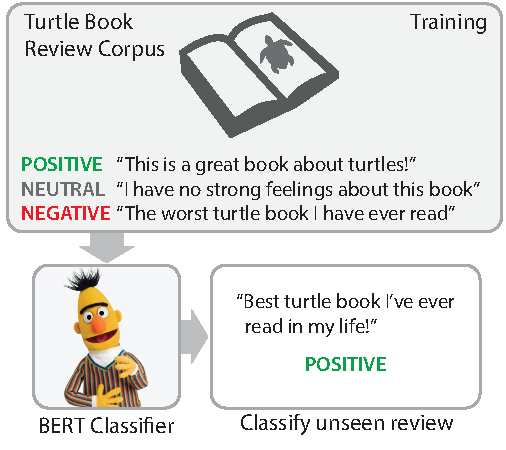
\includegraphics[scale=0.9]{turtle-figure.pdf}
%	\vspace{-20pt}
	\caption{\small An example of the sentiment analysis task.  A corpus of turtle book reviews serves as training data to fine-tune a BERT classification model, trained to classify reviews as \textit{positive, neutral,} or \textit{negative}.  The classifier is then evaluated on unseen reviews.}
	\label{fig:overview}}
	%\vspace{-14pt}
	\vspace{-4mm}
\end{figure}



The Introduction is typically 1-1.5 pages (i.e. may spill onto the first column of the second page).  The total length of your paper should follow the guideliens for a short ACL paper -- 4 pages, plus additional pages for references.  539 students may use 4 or 5 pages.

\todo{\lipsum[1-2]}



\section{Related Work}

In this section, provide a brief review of 3 papers that are related to your task.  Normally, this is where you review the state-of-the-art in this subfield or task, and briefly contrast it with your approach.  Here, you just need to identify 3 paper that are in the same area, and describe how they frame the task, what methods they use, and their main results.  Citations should be entered into the custom.bib file, and cited using the appropriate latex citation commands, e.g. \verb|\cite|.

Aho et al.~\shortcite{Aho:72} provided the first detailed study of sentiment analysis on turtle book reviews, where they use model XYZ on an in-house dataset of 50 turtle book reviews.  Compared to Aho et al.~\shortcite{Aho:72}, this work includes larger training evaluation, and uses fancy model 2.0 that improves ABC. 

Several groups have been interested in sentiment analysis on non-turtle books \cite[e.g.][]{Chandra:81,Gusfield:97}.  For example, Ando et al.~\shortcite{Ando2005} explore the related task of sentiment analysis on near-domain books such as lizard books, and pamphlets describing other reptiles.  etc. 

The related work should be approximately half a page. 

\todo{\lipsum[1]}

\section{Approach}

How do you frame the problem?  Classification, ranking, sequence2sequence, etc?  Do you need a figure to describe the actual task?  What are the important things to know about your task?  e.g. if it's classification, how many classes?

\todo{\lipsum[1]}

\subsection{Data collection}

Did you collect and/or label your own data for this task?  Describe the collection and labeling procedure here.  Provide one or two examples, possibly in a figure. 

Did you use someone elses data?  Describe it, and provide one or two examples, possibly in a figure. 

How is the data divided into train/dev/test sets? (e.g. 50\% / 25\% / 25\%)?

\todo{\lipsum[2]}

\subsection{Experiments}

We evaluate the performance of XX models.  Performance is measured using \textit{(How is your task evaluated?  Accuracy?  F1?  Precision@1?  etc. )}. 

\todo{\lipsum[2]}

\subsection{Models}

If you are doing an experimental paper, you must implement at least two models.  One model should be a ``baseline'' model -- a simple model that shows how well a simple method performs on the task.  Typically these are n-gram models (e.g. your unigram/bigram model using logistic regression from Assignment 2), ranking using tf.idf vectors, etc. 

{\flushleft\textbf{Model XYZ:}} Succinctly describe the workings of your baseline model here.  What features does it use?  What learning framework does it use?  etc. 
\todo{\lipsum[2]}

{\flushleft\textbf{Model ABC:}} Succinctly describe the workings of your other fancy model here. For example, we make use of a BERT-based classifier \cite{devlin2018bert} fine tuned to perform the sentiment analysis task.  For computational tractibility we make use of the TinyBERT \cite{jiao2020tinybert} classifier, which reduces BERT from a 110M parameter model to a XXM parameter model with reduced computational requirements, while retaining much of the performance benefits of the original model.  
\todo{\lipsum[2]}


%
%   Example Results Table
%
\begin{table}
\footnotesize
\centering
\begin{tabular}{lccc}
\toprule
\textbf{Model} & \textbf{Precision} & \textbf{Recall}   &   \textbf{F1}\\
\midrule
Baseline (Unigram+Bigram)     &       50      &   40      &   20      \\
Fancy Model 2.0                 &       60      &   50      &   30$^{\dagger}$      \\
\bottomrule
\end{tabular}
\caption{\label{tab:main-results}
Task performance across the models under investigation. $\dagger$ signifies that performance is significantly different from baseline performance ($p<0.05$) using a non-parametric bootstrap resampling test. }
\end{table}

\subsection{Hyperparameter Tuning}

You should report performance on both the \textbf{development} and \textbf{test} sets in your tables/figures, and describe any hyperparameters that were tuned on the development set.  

\subsection{Results}

The experiments are described in Table~\ref{tab:main-results}.  Overall the results show... 

\todo{\lipsum[1]}



\subsection{Error Analysis}

Students enrolled in 539 must complete an error analysis (and extend their papers into an additional page, to 5 pages).  Analyze 50-100 randomly picked errorful predictions that the model makes (on the development set), and distill them into a number of specific categories.  Those are shown in Table~\ref{tab:error-analysis} and described below. 

{\flushleft\textbf{Complex Examples (50\%):}} \todo{\lipsum[2]}

{\flushleft\textbf{Low frequency words (10\%):}}  \todo{\lipsum[2]}

{\flushleft\textbf{Sarcasm (5\%):}}  \todo{\lipsum[2]}

%
%   Example Error Analysis Table
%
\begin{table}
\footnotesize
\centering
\begin{tabular}{ll}
\toprule
\textbf{Prop.} & \textbf{Error Class}\\
\midrule
50\%    & Complex examples with ambiguous words\\
10\%    & Unseen data has low-frequency words \\
5\%     & Examples contain sarcasm \\
... \\
\bottomrule
\end{tabular}
\caption{\label{tab:error-analysis}
Common error classes and proportions of errors for 100 randomly selected errors on the development set.  }
\end{table}


\section{Conclusion}

A short summary paragraph (generally up to one third of one column) summarizing the results. 
\todo{\lipsum[2]}

\section{Project Site}

The project is available at \url{http://www.github.com/...} .


% Entries for the entire Anthology, followed by custom entries
\bibliography{anthology,custom}
\bibliographystyle{acl_natbib}

\appendix

\section{Example Appendix}
\label{sec:appendix}

This is an appendix.

\end{document}
